\documentclass[12pt,a4paper]{article}

% ─── Page Layout ───────────────────────────────────────────────────────────────
\usepackage[a4paper, margin=0.8in, headheight=14pt]{geometry}

% ─── Fonts (XeLaTeX) ───────────────────────────────────────────────────────────
\usepackage{fontspec}
\usepackage{unicode-math}
\setmainfont{TeX Gyre Pagella}
\setmonofont[Scale=0.88]{TeX Gyre Cursor}
\setmathfont{Latin Modern Math}

% ─── Packages ──────────────────────────────────────────────────────────────────
\usepackage{xcolor}
\usepackage{colortbl}
\usepackage{titlesec}
\usepackage{enumitem}
\usepackage{tabularx}
\usepackage{booktabs}
\usepackage{array}
\usepackage{amsmath}
\usepackage{tikz}
\usetikzlibrary{shapes.geometric, arrows.meta, positioning, calc, fit, decorations.pathreplacing}
\usepackage{tcolorbox}
\tcbuselibrary{skins, breakable}
\usepackage{hyperref}
\usepackage{fancyhdr}
\usepackage{graphicx}
\usepackage{microtype}
\hyphenpenalty=10000
\exhyphenpenalty=10000
\sloppy
\usepackage{caption}
\usepackage{setspace}
\usepackage{multirow}
\usepackage{tocloft}

% ─── Q&A helper ────────────────────────────────────────────────────────────────
\newcommand{\Q}[1]{\textbf{#1}\par\noindent\ignorespaces}

% ─── Colour Palette ────────────────────────────────────────────────────────────
\definecolor{myred}{RGB}{196,30,58}
\definecolor{mydark}{RGB}{30,30,50}
\definecolor{mygreen}{RGB}{14,120,80}
\definecolor{myteal}{RGB}{0,130,140}
\definecolor{myamber}{RGB}{180,100,0}
\definecolor{mypurple}{RGB}{100,30,160}
\definecolor{mygray}{RGB}{246,247,249}
\definecolor{mgframe}{RGB}{180,185,200}
\definecolor{watermark}{RGB}{145,150,170}
\definecolor{hdrred}{RGB}{250,232,235}
\definecolor{hdrgreen}{RGB}{220,244,233}
\definecolor{hdrteal}{RGB}{220,242,244}
\definecolor{hdramber}{RGB}{253,242,215}
\definecolor{hdrpurple}{RGB}{238,228,255}
\definecolor{hdrgray}{RGB}{238,240,245}
\definecolor{rowalt}{RGB}{250,251,253}

% ─── Section Formatting ────────────────────────────────────────────────────────
\titleformat{\section}
  {\large\bfseries\color{myred}}{\thesection.}{0.5em}{}
  [\vspace{1pt}{\color{myred}\rule{\linewidth}{0.8pt}}]
\titleformat{\subsection}
  {\normalsize\bfseries\color{myteal}}{\thesubsection}{0.5em}{}
\titlespacing*{\section}{0pt}{18pt}{7pt}
\titlespacing*{\subsection}{0pt}{11pt}{4pt}

% ─── Paragraph ─────────────────────────────────────────────────────────────────
\setlength{\parindent}{0pt}
\setlength{\parskip}{4pt}

% ─── TOC Styling ───────────────────────────────────────────────────────────────
\renewcommand{\cfttoctitlefont}{\large\bfseries\color{myred}}
\renewcommand{\cftaftertoctitle}{\par\noindent{\color{myred}\rule{\linewidth}{0.8pt}}}
\setlength{\cftbeforetoctitleskip}{0pt}
\setlength{\cftaftertoctitleskip}{6pt}
\renewcommand{\cftsecfont}{\normalsize\bfseries\color{mydark}}
\renewcommand{\cftsecpagefont}{\normalsize\bfseries\color{mydark}}
\renewcommand{\cftsecleader}{\cftdotfill{\cftdotsep}}
\setlength{\cftbeforesecskip}{7pt}
\renewcommand{\cftsubsecfont}{\small\color{mydark}}
\renewcommand{\cftsubsecpagefont}{\small\color{mydark}}
\setlength{\cftbeforesubsecskip}{3pt}
\setlength{\cftsubsecindent}{1.4em}

% ─── Table helpers ─────────────────────────────────────────────────────────────
\renewcommand{\arraystretch}{1.45}
\setlength{\tabcolsep}{6pt}
\arrayrulecolor{mydark}
\newcolumntype{B}[1]{>{\small\bfseries\raggedright\arraybackslash}m{#1}}
\newcolumntype{Y}{>{\small\raggedright\arraybackslash}X}
\renewcommand{\tabularxcolumn}[1]{m{#1}}

% ─── Header / Footer ───────────────────────────────────────────────────────────
\pagestyle{fancy}
\fancyhf{}
\fancyhead[L]{\small\color{myred}\textbf{PE-EC701A}\;\color{mydark}--- Microwave Theory and Technique}
\fancyhead[R]{\small\color{myteal}\textbf{Module 5 Notes}}
\fancyfoot[C]{\small\color{mydark}\thepage}
\fancyfoot[R]{\small\color{watermark}\textit{\copyright\ Biraj}}
\renewcommand{\headrulewidth}{0.5pt}
\renewcommand{\footrulewidth}{0.3pt}

% ─── Hyperref ──────────────────────────────────────────────────────────────────
\hypersetup{
  colorlinks=true, linkcolor=myteal, urlcolor=myteal,
  pdfauthor={Biraj Sarkar},
  pdftitle={PE-EC701A --- Module 5 Notes}
}

% ─── tcolorbox styles ──────────────────────────────────────────────────────────
\tcbset{
  tikzbox/.style={
    colback=mygray, colframe=mgframe, boxrule=0.6pt, arc=4pt,
    left=8pt, right=8pt, top=6pt, bottom=6pt,
    colbacktitle=mgframe, coltitle=mydark,
    fonttitle=\small\bfseries
  },
  defbox/.style={
    colback=hdrgreen, colframe=mygreen, boxrule=0.8pt, arc=4pt,
    left=9pt, right=9pt, top=6pt, bottom=6pt,
    colbacktitle=mygreen, coltitle=white,
    fonttitle=\small\bfseries
  },
  formulabox/.style={
    colback=hdrteal, colframe=myteal, boxrule=0.8pt, arc=4pt,
    left=9pt, right=9pt, top=7pt, bottom=7pt,
    colbacktitle=myteal, coltitle=white,
    fonttitle=\small\bfseries
  },
  examplebox/.style={
    colback=hdramber, colframe=myamber, boxrule=0.8pt, arc=4pt,
    left=9pt, right=9pt, top=6pt, bottom=6pt,
    colbacktitle=myamber, coltitle=white,
    fonttitle=\small\bfseries
  },
  masonbox/.style={
    colback=hdrpurple, colframe=mypurple, boxrule=0.8pt, arc=4pt,
    left=9pt, right=9pt, top=6pt, bottom=6pt,
    colbacktitle=mypurple, coltitle=white,
    fonttitle=\small\bfseries
  },
  exambox/.style={
    colback=hdrpurple, colframe=mypurple, boxrule=1pt, arc=5pt,
    left=10pt, right=10pt, top=8pt, bottom=8pt,
    colbacktitle=mypurple, coltitle=white,
    fonttitle=\bfseries,
    breakable, title after break={\textbf{Frequently Asked / Viva Questions (contd.)}}}
}
% Make all boxes breakable across pages
\tcbset{breakable}

% ─── TikZ styles ───────────────────────────────────────────────────────────────
\tikzset{
  block/.style={rectangle, draw=myteal, fill=hdrteal,
    text width=2.4cm, align=center, minimum height=0.95cm,
    font=\small, rounded corners=3pt, line width=0.7pt},
  redblock/.style={rectangle, draw=myred, fill=hdrred,
    text width=2.4cm, align=center, minimum height=0.95cm,
    font=\small, rounded corners=3pt, line width=0.7pt},
  netnode/.style={rectangle, draw=myteal, fill=hdrteal,
    text width=1.5cm, align=center, minimum height=0.8cm,
    font=\small, rounded corners=3pt, line width=0.7pt},
  sumjunc/.style={circle, draw=myamber, fill=hdramber,
    minimum size=0.62cm, font=\small, line width=0.8pt},
  snode/.style={circle, draw=mypurple, fill=hdrpurple,
    minimum size=0.55cm, font=\footnotesize, line width=0.7pt},
  arrow/.style={-Stealth, thick, color=mydark},
  redarrow/.style={-Stealth, thick, color=myred},
  line/.style={thick, color=mydark}
}

% ═══════════════════════════════════════════════════════════════════════════════
\begin{document}
% ═══════════════════════════════════════════════════════════════════════════════

\begin{center}
  {\LARGE\bfseries\color{myred} PE-EC701A --- Microwave Theory and Technique}\\[5pt]
  {\normalsize\color{mydark} Semester VII \quad$\bullet$\quad 3L:0T:0P \quad$\bullet$\quad 3 Credits}\\[3pt]
  {\normalsize\color{myteal}\textbf{Module 5 Exam Notes: Passive and Active Microwave Devices}}\\[3pt]
  {\small\color{mydark} CGEC \;$|$\; B.Tech ECE (2023--27) \;$|$\; \textit{Biraj Sarkar}}
\end{center}
\vspace{2pt}
\noindent{\color{myred}\rule{\linewidth}{1.5pt}}
\vspace{2pt}

\hypersetup{linkcolor=mydark}
\tableofcontents
\hypersetup{linkcolor=myteal}
\newpage

% ===============================================================================
\section{Microwave Passive Components}
% ===============================================================================

Microwave passive components route, split, attenuate, or filter RF signals without adding energy to the system.

\subsection{Directional Coupler}
A directional coupler is a 4-port device that couples a specific fraction of power from one transmission line to another in a directive manner.
\begin{itemize}[leftmargin=*, itemsep=3pt]
  \item \textbf{Port 1 (Input), Port 2 (Through), Port 3 (Coupled), Port 4 (Isolated).}
  \item \textbf{Key Parameters:} Coupling ($C$), Directivity ($D$), and Isolation ($I$).
\end{itemize}

\begin{tcolorbox}[formulabox, title={\textbf{Directional Coupler Metrics \& S-Matrix}}]
\begin{align}
  \text{Coupling Factor } C &= -20 \log_{10} \left| \frac{P_3}{P_1} \right| \quad (\text{dB}) \\
  \text{Directivity } D &= -20 \log_{10} \left| \frac{P_4}{P_3} \right| \quad (\text{dB}) \\
  \text{Isolation } I &= -20 \log_{10} \left| \frac{P_4}{P_1} \right| = C + D \quad (\text{dB})
\end{align}
The S-matrix of an ideal symmetric reciprocal coupler (normalized to matched ports) is:
\begin{equation}
  [S] = \begin{bmatrix} 0 & p & j q & 0 \\ p & 0 & 0 & j q \\ j q & 0 & 0 & p \\ 0 & j q & p & 0 \end{bmatrix} \quad (\text{with } p^2 + q^2 = 1)
\end{equation}
\end{tcolorbox}

\subsection{Magic Tee (Hybrid Tee)}
A Magic Tee is a 4-port waveguide junction combining an E-plane (series) arm and an H-plane (shunt) arm. It is used as a mixer or duplexer.

\begin{tcolorbox}[tikzbox, title={Magic Tee Port Configuration Scheme}]
\begin{minipage}[c]{0.45\linewidth}
\centering
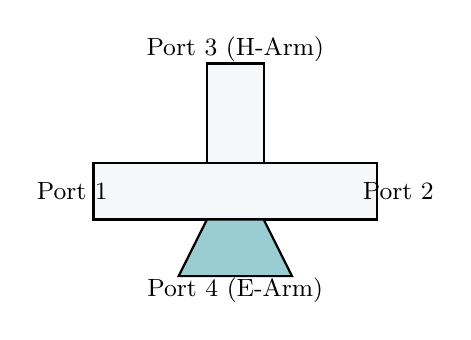
\begin{tikzpicture}[scale=0.9, every node/.style={font=\small}]
  % Drawing Magic Tee schematic representation
  \draw[thick, fill=mygray] (-2,-0.4) rectangle (2,0.4);
  \draw[thick, fill=mygray] (-0.4,0.4) rectangle (0.4,1.8); % H-plane arm
  \draw[thick, fill=myteal!40] (-0.4,-0.4) -- (-0.8,-1.2) -- (0.8,-1.2) -- (0.4,-0.4) -- cycle; % E-plane arm (projected down)
  
  \node at (-2.3,0) {Port 1};
  \node at (2.3,0) {Port 2};
  \node at (0,2.0) {Port 3 (H-Arm)};
  \node at (0,-1.4) {Port 4 (E-Arm)};
\end{tikzpicture}
\end{minipage}\hfill
\begin{minipage}[c]{0.5\linewidth}
\raggedright
\textbf{Operation:}\\[3pt]
$\bullet$ Feed Port 3 $\to$ Outputs 1 \& 2 in-phase ($V_1 = V_2$)\\[2pt]
$\bullet$ Feed Port 4 $\to$ Outputs 1 \& 2 out-of-phase ($V_1 = -V_2$)\\[2pt]
$\bullet$ Feed Port 1 \& 2 $\to$ Sum at Port 3, Diff at Port 4
\end{minipage}
\end{tcolorbox}

\begin{tcolorbox}[formulabox, title={\textbf{Magic Tee S-Matrix}}]
For matched and isolated E and H ports:
\begin{equation}
  [S] = \frac{1}{\sqrt{2}} \begin{bmatrix} 0 & 0 & 1 & 1 \\ 0 & 0 & 1 & -1 \\ 1 & 1 & 0 & 0 \\ 1 & -1 & 0 & 0 \end{bmatrix}
\end{equation}
\end{tcolorbox}

\subsection{Waveguide Attenuators}
Microwave attenuators are passive components used to reduce the amplitude or power level of a signal by a desired amount (expressed in dB) while maintaining impedance matching.
\begin{itemize}[leftmargin=*, itemsep=3pt]
  \item \textbf{Fixed Attenuator:} Employs a thin resistive card placed at the center of the waveguide parallel to the maximum electric field ($TE_{10}$ mode). It absorbs RF energy and dissipates it as heat.
  \item \textbf{Rotary Vane Variable Attenuator:} Consists of three sections: a center circular waveguide containing a rotatable resistive card, positioned between two rectangular-to-circular transitions with fixed horizontal cards.
  \begin{itemize}[leftmargin=*, itemsep=2.5pt, topsep=0pt]
    \item When the center card is rotated by an angle $\theta$ relative to the incoming E-field, the parallel component is absorbed. The perpendicular component ($E \cos\theta$) passes.
    \item Passing through the output transition (which is horizontal), the field is further reduced by $\cos\theta$, resulting in an output amplitude of $E_0 = E \cos^2\theta$.
    \item \textbf{Attenuation Equation:}
      \begin{equation}
        A_{\text{dB}} = -20 \log_{10}(\cos^2\theta) = -40 \log_{10}(\cos\theta)
      \end{equation}
      This attenuation depends strictly on rotation angle $\theta$, making it highly precise and frequency-independent.
  \end{itemize}
\end{itemize}

\subsection{Power Divider (T-Junction and Wilkinson)}
Power dividers are passive 3-port networks used to split an input signal into two or more output signals of lesser power.
\begin{itemize}[leftmargin=*, itemsep=3pt]
  \item \textbf{Reciprocal Lossless 3-Port Limitation:} By S-matrix properties, it is mathematically impossible for a 3-port junction to be simultaneously reciprocal, lossless, and matched at all ports.
  \item \textbf{T-Junction Power Divider:} A simple lossless reciprocal 3-port divider (E-plane or H-plane waveguide junction or microstrip line). Since it is lossless and reciprocal, it cannot be matched at all ports simultaneously (typically the output ports are mismatched, leading to reflections).
  \item \textbf{Wilkinson Power Divider:} A reciprocal 3-port network that achieves matching at all ports simultaneously and provides high isolation between the output ports by utilizing internal loss under mismatch. It is lossless when the output ports are matched and balanced.
\end{itemize}

\begin{tcolorbox}[tikzbox, title={Wilkinson Power Divider Transmission Line Layout}]
\centering
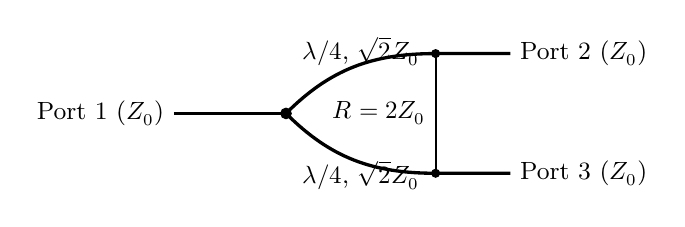
\begin{tikzpicture}[scale=0.95, every node/.style={font=\small}]
  % Input line
  \draw[very thick] (0,0) -- (1.5,0);
  \node[left] at (0,0) {Port 1 ($Z_0$)};
  
  % Split junction
  \filldraw (1.5,0) circle (2pt);
  
  % Upper branch (quarter-wave transformer)
  \draw[very thick] (1.5,0) to[out=45, in=180] (3.5,0.8) -- (4.5,0.8);
  \node[above] at (2.5,0.5) {$\lambda/4$, $\sqrt{2}Z_0$};
  \node[right] at (4.5,0.8) {Port 2 ($Z_0$)};
  
  % Lower branch (quarter-wave transformer)
  \draw[very thick] (1.5,0) to[out=-45, in=180] (3.5,-0.8) -- (4.5,-0.8);
  \node[below] at (2.5,-0.5) {$\lambda/4$, $\sqrt{2}Z_0$};
  \node[right] at (4.5,-0.8) {Port 3 ($Z_0$)};
  
  % Isolation Resistor
  \draw[thick] (3.5,0.8) -- (3.5,-0.8);
  \filldraw (3.5,0.8) circle (1.5pt);
  \filldraw (3.5,-0.8) circle (1.5pt);
  \node[left] at (3.5,0) {$R = 2Z_0$};
\end{tikzpicture}
\end{tcolorbox}

\begin{tcolorbox}[formulabox, title={\textbf{Wilkinson Power Divider S-Matrix}}]
For design parameters with quarter-wave line impedance of $Z_0\sqrt{2}$ and an isolation resistor of $2Z_0$, the S-matrix of an ideal symmetric Wilkinson power divider matched at all three ports is:
\begin{equation}
  [S] = -\frac{j}{\sqrt{2}} \begin{bmatrix} 0 & 1 & 1 \\ 1 & 0 & 0 \\ 1 & 0 & 0 \end{bmatrix}
\end{equation}
When ports 2 and 3 are matched, no current flows through the isolation resistor $2Z_0$, and the power is split equally with zero loss ($S_{21} = S_{31} = -3\text{ dB}$).
\end{tcolorbox}

\subsection{Cavity Resonators}
A microwave cavity resonator is a metallic enclosure that confines electromagnetic energy inside a cavity, storing it in standing waves.
\begin{itemize}[leftmargin=*, itemsep=3pt]
  \item \textbf{Mechanism:} Unlike lumped LC circuits which suffer from high radiation and conductor losses at gigahertz frequencies, cavity resonators completely enclose fields to achieve extremely high Q-factors ($10^3$ to $10^5$).
  \item \textbf{Rectangular Cavity Resonator:} Formed by closing both ends of a rectangular waveguide of dimensions $a \times b$ at a distance $d$ (along the z-axis). Resonance occurs when the guide length $d$ is an integer multiple of half-guide-wavelengths ($d = p \lambda_g / 2$).
\end{itemize}

\begin{tcolorbox}[formulabox, title={\textbf{Cavity Resonance \& Quality Factor}}]
The resonant frequency $f_{mnp}$ for $\text{TE}_{mnp}$ or $\text{TM}_{mnp}$ modes in a rectangular cavity filled with dielectric ($\epsilon_r$) is:
\begin{equation}
  f_{mnp} = \frac{c}{2\sqrt{\epsilon_r}} \sqrt{\left(\frac{m}{a}\right)^{\!2} + \left(\frac{n}{b}\right)^{\!2} + \left(\frac{p}{d}\right)^{\!2}} \quad (\text{Hz})
\end{equation}
The \textbf{Quality Factor ($Q$)} measures the energy storage efficiency of the resonator:
\begin{equation}
  Q = 2\pi \frac{\text{Energy Stored}}{\text{Energy Dissipated per cycle}} = \omega \frac{W}{P_L}
\end{equation}
\begin{itemize}[leftmargin=1.5em, itemsep=2pt, topsep=2pt]
  \item \textbf{Unloaded $Q$ ($Q_0$):} Internal $Q$ of the cavity itself, accounting for conductor wall losses ($Q_c$) and dielectric losses ($Q_d$): $1/Q_0 = 1/Q_c + 1/Q_d$.
  \item \textbf{Loaded $Q$ ($Q_L$):} Accounts for both internal cavity losses and external circuit load losses ($Q_e$):
    \begin{equation}
      \frac{1}{Q_L} = \frac{1}{Q_0} + \frac{1}{Q_e}
    \end{equation}
\end{itemize}
\end{tcolorbox}

% ===============================================================================
\section{Microwave Semiconductor Devices}
% ===============================================================================

\subsection{Gunn Diode}
The Gunn diode is not a junction diode but a bulk semiconductor device (typically GaAs) that exhibits negative differential resistance due to the \textbf{transferred-electron mechanism (RWH Theory)}.
\begin{itemize}[leftmargin=*, itemsep=3pt]
  \item Under high electric fields, electrons transfer from a high-mobility lower valley to a low-mobility upper valley in the conduction band, causing current to drop as voltage increases.
\end{itemize}

\subsection{IMPATT Diode}
The \textbf{IMPATT (IMPact ionization Avalanche Transit Time)} diode operates under reverse breakdown, utilizing avalanche multiplication and carrier transit time delays to generate a $180^\circ$ phase shift (negative resistance) at microwave frequencies.

\subsection{PIN Diode}
Constructed with a high-resistivity intrinsic semiconductor sandwiched between p-type and n-type regions.
\begin{itemize}[leftmargin=*, itemsep=3pt]
  \item \textbf{Under Forward Bias:} Behaves as a low-resistance resistor ($\sim 1\,\Omega$), passing RF.
  \item \textbf{Under Reverse Bias:} Behaves as a high resistance in parallel with a small capacitance, blocking RF. Ideal as a high-speed RF switch.
\end{itemize}

\subsection{Schottky Barrier Diode}
The Schottky barrier diode consists of a metal-semiconductor rectifying junction (e.g., gold or tungsten on n-type GaAs).
\begin{itemize}[leftmargin=*, itemsep=3pt]
  \item \textbf{Working:} Unlike standard p-n diodes, it is a \textbf{majority carrier device}. When forward-biased, electrons from the semiconductor are injected into the metal (thermionic emission) where they rapidly lose energy.
  \item \textbf{High-Frequency Advantage:} Since there is \textbf{zero minority carrier storage time} (no charge storage delay), the diode can switch states in picoseconds, making it ideal for low-noise mixers, detectors, and switching circuits up to THz frequencies.
\end{itemize}

\subsection{GaAs MESFET}
The Metal-Semiconductor Field Effect Transistor (MESFET) replaces the traditional insulated gate of a MOSFET with a metal Schottky barrier gate deposited directly on an n-type GaAs channel.
\begin{itemize}[leftmargin=*, itemsep=3pt]
  \item \textbf{Operation:} Gate voltage modulates the depletion region width beneath the Schottky gate, controlling channel conduction.
  \item \textbf{Key Feature:} The high electron mobility of GaAs (compared to Silicon) yields extremely high electron drift velocities, enabling high cut-off frequencies ($f_T > 100\,\text{GHz}$).
\end{itemize}

\subsection{HEMT (High Electron Mobility Transistor)}
The HEMT (or MODFET) is a heterostructure field-effect transistor that utilizes the junction between materials of different bandgaps (e.g., AlGaAs and GaAs).
\begin{itemize}[leftmargin=*, itemsep=3pt]
  \item \textbf{2DEG formation:} Free electrons from the n-doped AlGaAs layer migrate across the heterojunction to the undoped GaAs side, where they are trapped in a quantum well, forming a thin sheet of charge called a \textbf{Two-Dimensional Electron Gas (2DEG)}.
  \item \textbf{Carrier Mobility:} Because the 2DEG channel lies in an undoped GaAs layer, the moving electrons experience \textbf{no ionized impurity scattering}. This results in extremely high carrier mobilities and noise figures near zero, making HEMTs the industry standard for Low Noise Amplifiers (LNAs).
\end{itemize}

% ===============================================================================
\section{Microwave Tubes (Linear-Beam and Cross-Field)}
% ===============================================================================

Traditional vacuum tubes fail at microwave frequencies due to \textbf{transit-time effects} (the time taken by electrons to cross the grid becomes comparable to the RF cycle period, causing grid loading). Microwave tubes overcome this by utilizing electron velocity modulation.

\subsection{Klystron (Two-Cavity and Reflex)}
In a Two-Cavity Klystron, an electron beam passes through a \textbf{buncher cavity} where a small RF signal velocity-modulates the electrons (speeding up some, slowing down others). During travel through the drift space, they form \textbf{bunches} that yield strong RF currents in the \textbf{catcher cavity}.

\begin{tcolorbox}[tikzbox, title={Applegate Diagram of Velocity Modulation}]
\centering
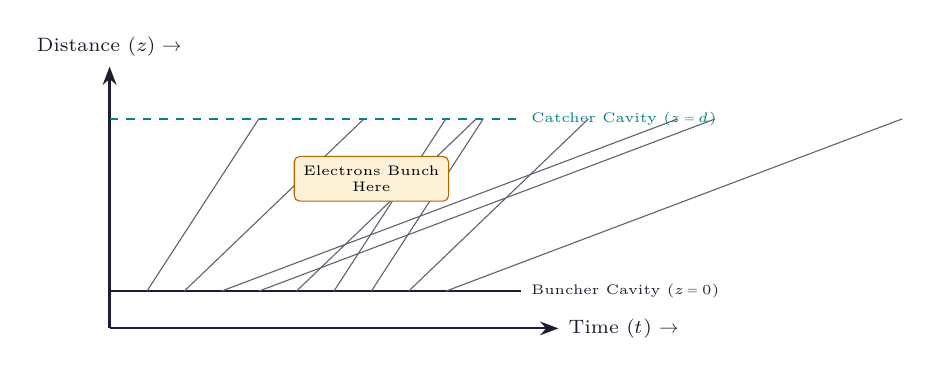
\begin{tikzpicture}[scale=0.95]
  \draw[arrow] (0,0) -- (6,0) node[right, font=\scriptsize] {Time ($t$) $\to$};
  \draw[arrow] (0,0) -- (0,3.5) node[above, font=\scriptsize] {Distance ($z$) $\to$};
  
  % Buncher position
  \draw[line] (0,0.5) -- (5.5,0.5) node[right, font=\tiny\color{myred}] {Buncher Cavity ($z=0$)};
  \draw[line, dashed, color=myteal] (0,2.8) -- (5.5,2.8) node[right, font=\tiny\color{myteal}] {Catcher Cavity ($z=d$)};
  
  % Electron paths (slopes represent velocities)
  \foreach \t in {0.5, 1.0, 1.5, 2.0, 2.5, 3.0, 3.5, 4.0, 4.5} {
    % Modulate slope based on sin function of start time
    \pgfmathsetmacro{\slope}{0.5 + 0.35*sin((\t-2.5)*180/1.5)}
    \draw[color=mydark!70, thin] (\t, 0.5) -- (\t + 1.2/\slope, 2.8);
  }
  
  \node[draw=myamber, fill=hdramber, rounded corners=2pt, font=\tiny, align=center] at (3.5,2.0) {Electrons Bunch\\Here};
\end{tikzpicture}
\end{tcolorbox}

\textbf{Reflex Klystron:} Uses a single cavity and a \textbf{repeller electrode} to return electrons back through the cavity, creating feedback and oscillation.

\subsection{Traveling Wave Tube (TWT)}
A TWT is a non-resonant linear amplifier. It utilizes a \textbf{slow-wave structure} (usually a wire helix) to slow down the RF wave phase velocity so it matches the electron beam velocity, allowing continuous energy transfer along the entire tube length.

\begin{tcolorbox}[tikzbox, title={Traveling Wave Tube (TWT) Concept}]
\centering
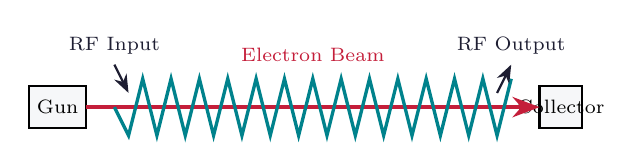
\begin{tikzpicture}[scale=0.9, every node/.style={font=\scriptsize}]
  % Electron Gun
  \draw[thick, fill=mygray] (0,0.4) rectangle (0.8,1.0) node[midway] {Gun};
  % Collector
  \draw[thick, fill=mygray] (7.2,0.4) rectangle (7.8,1.0) node[midway] {Collector};
  
  % Electron Beam
  \draw[line width=1.5pt, color=myred, -Stealth] (0.8,0.7) -- (7.2,0.7);
  \node[above, color=myred, font=\scriptsize] at (4,1.2) {Electron Beam};
  
  % Helix line (slow wave structure)
  \draw[very thick, color=myteal] (1.2,0.7) 
    \foreach \x in {1.4,1.8,2.2,2.6,3.0,3.4,3.8,4.2,4.6,5.0,5.4,5.8,6.2,6.6} {
      -- (\x, 0.3) -- (\x+0.2, 1.1)
    };
    
  \draw[arrow] (1.2,1.3) node[above] {RF Input} -- (1.4,0.9);
  \draw[arrow] (6.6,0.9) -- (6.8,1.3) node[above] {RF Output};
\end{tikzpicture}
\end{tcolorbox}

\subsection{Magnetron}
A cavity magnetron is a high-power cross-field (M-type) microwave oscillator.
\begin{itemize}[leftmargin=*, itemsep=3pt]
  \item \textbf{Crossed Fields:} Direct electric field ($\vec{E}$) between anode and cathode, and axial magnetic field ($\vec{B}$) perpendicular to the electric field.
  \item \textbf{Working:} Electrons from the cathode spiral in the crossed fields, interacting with the resonant cavities in the anode block. In the \textbf{$\pi$-mode}, adjacent cavities oscillate $180^\circ$ out-of-phase, forcing electrons into spokes that continuously feed energy to the cavities.
\end{itemize}

\begin{tcolorbox}[tikzbox, title={Cavity Magnetron Cross-Section}]
\begin{minipage}[c]{0.45\linewidth}
\centering
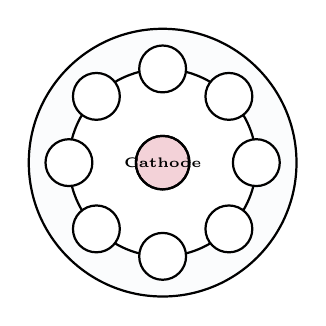
\begin{tikzpicture}[scale=0.85]
  % Outer anode ring
  \draw[thick, fill=mygray!40] (0,0) circle (2.0cm);
  \draw[thick, fill=white] (0,0) circle (1.4cm);
  
  % Inner cathode
  \draw[thick, fill=myred!20] (0,0) circle (0.4cm);
  \node[font=\tiny\bfseries] at (0,0) {Cathode};
  
  % 8 Cavities
  \foreach \angle in {0, 45, 90, 135, 180, 225, 270, 315} {
    \draw[thick, fill=white] (\angle:1.4) circle (0.35cm);
  }
  
  % Re-draw cathode outline
  \draw[thick] (0,0) circle (0.4cm);
\end{tikzpicture}
\end{minipage}\hfill
\begin{minipage}[c]{0.5\linewidth}
\raggedright
$\bullet$ \textbf{Anode Block:} 8 Cavities\\[3pt]
$\bullet$ \textbf{Crossed Fields:} $\vec{E}$ radial, $\vec{B}$ perpendicular to page ($\odot$)\\[3pt]
$\bullet$ Electrons form rotating "spokes"
\end{minipage}
\end{tcolorbox}

% ===============================================================================
% MANDATORY QUICK REVISION PAGE
% ===============================================================================
\newpage
\begin{center}
  {\large\bfseries\color{myred} Quick Revision --- Module V}\\[3pt]
  {\small\color{mydark} Passive and Active Microwave Devices $|$ PE-EC701A}
\end{center}
\noindent{\color{myred}\rule{\linewidth}{1.2pt}}
\vspace{4pt}

\begin{tcolorbox}[formulabox, title={\textbf{Key Formulas at a Glance}}]
\renewcommand{\arraystretch}{1.3}
\begin{tabularx}{\linewidth}{B{4.5cm} X}
Coupling Factor ($C$)   & $C = -20 \log_{10} |S_{31}| = -20 \log_{10} |P_3/P_1|^{1/2}$ \\[4pt]
Directivity ($D$)       & $D = -20 \log_{10} |S_{43}| = -20 \log_{10} |P_4/P_3|^{1/2}$ \\[4pt]
Isolation ($I$)         & $I = C + D = -20 \log_{10} |S_{41}|$ \\[4pt]
Wilkinson S-matrix      & $[S] = -\frac{j}{\sqrt{2}} \begin{bmatrix} 0 & 1 & 1 \\ 1 & 0 & 0 \\ 1 & 0 & 0 \end{bmatrix}$ \\[4pt]
Resonator frequency     & $f_0 = \frac{c}{2\sqrt{\epsilon_r}} \sqrt{(m/a)^2 + (n/b)^2 + (p/d)^2}$ \\[4pt]
Rotary Vane Attenuation & $A_{\text{dB}} = -40 \log_{10}(\cos\theta)$
\end{tabularx}
\tcbset{colbacktitle=mygreen, coltitle=white}
\end{tcolorbox}

\begin{tcolorbox}[defbox, title={\textbf{One-Line Definitions}}]
\begin{itemize}[leftmargin=*, itemsep=2.5pt, topsep=0pt]
  \item \textbf{Magic Tee:} A 4-port waveguide hybrid junction combining E and H arms to perform sum and difference processing.
  \item \textbf{Gunn Effect:} The emission of coherent microwave oscillations from bulk semiconductor material under high fields.
  \item \textbf{Negative Resistance:} A device property where current decreases with increasing voltage, enabling amplification.
  \item \textbf{Transit Time:} The time taken by a charge carrier to traverse the active length of a device.
  \item \textbf{Slow-Wave Structure:} A wire helix or waveguide circuit that reduces RF phase velocity to match electron beam speed.
  \item \textbf{Bunching:} The process in microwave tubes where velocity-modulated electrons form spatial charge clusters.
  \item \textbf{Applegate Diagram:} A distance-time graphical plot showing electron bunching trajectories in klystrons.
  \item \textbf{Schottky Diode:} A metal-semiconductor junction diode relying on majority carriers for zero reverse recovery delay.
  \item \textbf{GaAs MESFET:} Field-effect transistor using a Schottky barrier metal gate directly on a GaAs channel.
  \item \textbf{HEMT:} High Electron Mobility Transistor; uses a heterojunction to form a high-speed, low-noise 2DEG layer.
  \item \textbf{Rotary Vane Attenuator:} A frequency-independent waveguide attenuator calibrated via a rotating resistive vane.
\end{itemize}
\end{tcolorbox}

\begin{tcolorbox}[exambox, title={\textbf{Frequently Asked / Viva Questions}}]
\begin{enumerate}[topsep=0pt, label=\textbf{Q\arabic*.}, itemsep=5pt]
  \item \Q{State the matching and isolation properties of a Magic Tee.}
    If ports 3 (H-port) and 4 (E-port) are matched, they are isolated from each other ($S_{34} = S_{43} = 0$). Additionally, collinear ports 1 and 2 are isolated from each other ($S_{12} = S_{21} = 0$).
  \item \Q{Why are conventional triodes and pentodes useless at microwave frequencies?}
    Due to transit-time effects and lead inductance/capacitance, which cause severe grid loading and phase shifts that prevent amplification.
  \item \Q{Explain the basic principle of velocity modulation in a Klystron.}
    The input RF voltage in the buncher cavity accelerates electrons during the positive half-cycle and decelerates them during the negative half-cycle, converting a uniform velocity beam into a velocity-modulated beam.
  \item \Q{How does a TWT differ from a Klystron?}
    A Klystron uses resonant cavities for narrow-band interaction, while a TWT uses a non-resonant slow-wave structure (helix) for wide-band continuous interaction.
  \item \Q{What are the roles of the crossed fields in a Cavity Magnetron?}
    The radial electric field accelerates electrons. The axial magnetic field forces them into circular paths. Together, they form a rotating charge cloud that feeds energy to the cavities.
  \item \Q{Why is a Gunn diode referred to as a Transfer Electron Device (TED)?}
    Because it generates negative resistance by transferring conduction electrons from a high-mobility lower energy valley to a low-mobility higher energy valley.
  \item \Q{Explain the function of a PIN diode as an RF switch.}
    Forward bias injects carriers into the intrinsic layer, creating a low resistance path (closed switch). Reverse bias leaves the intrinsic layer depleted, showing high impedance (open switch).
  \item \Q{What is the Wilkinson Power Divider and what is its S-matrix?}
    It is a lossless 3-port divider that splits input power equally between ports 2 and 3 in-phase while providing isolation between them.
  \item \Q{What does the $\pi$-mode represent in a Magnetron?}
    It represents the operational state where adjacent anode cavities oscillate with a phase difference of $180^\circ$ ($\pi$ radians), which is the most stable and efficient mode.
  \item \Q{State the primary disadvantage of IMPATT diodes.}
    They generate high levels of avalanche phase noise due to the statistical/random nature of the impact ionization process.
  \item \Q{What is the function of the repeller in a Reflex Klystron?}
    It has a negative potential that repels the velocity-modulated electron beam, forcing it to turn back and bunch, feeding energy back into the single cavity to sustain oscillation.
  \item \Q{Why are cavity resonators preferred over lumped LC circuits at microwave frequencies?}
    Because lumped LC circuits have extremely high radiative losses and low Q-factors at GHz frequencies. Cavity resonators confine fields completely, achieving Q-factors in the thousands.
  \item \Q{Why does a Schottky barrier diode have a higher cutoff frequency than a p-n junction diode?}
    Because it is a majority carrier device, which eliminates the minority carrier injection and storage time (reverse recovery time) during switching. This enables it to operate up to THz frequencies.
  \item \Q{Explain the formation of a 2DEG in a HEMT. Why is its electron mobility so high?}
    A 2DEG (Two-Dimensional Electron Gas) forms at the heterojunction of AlGaAs and GaAs, where electrons drop into a thin GaAs quantum well. The mobility is extremely high because the GaAs channel is undoped, eliminating ionized impurity scattering.
  \item \Q{Prove that the attenuation of a rotary vane attenuator is given by $-40 \log_{10}(\cos\theta)$.}
    An input E-field component parallel to the rotating card ($E\sin\theta$) is absorbed, leaving $E\cos\theta$ aligned with it. Reaching the horizontal output transition card, only its horizontal component is transmitted: $E_{\text{out}} = (E\cos\theta)\cos\theta = E\cos^2\theta$. The power attenuation ratio is $P_{\text{out}}/P_{\text{in}} = (E_{\text{out}}/E)^2 = \cos^4\theta$. Thus, $A_{\text{dB}} = -10 \log_{10}(\cos^4\theta) = -40 \log_{10}(\cos\theta)$.
\end{enumerate}
\tcbset{colbacktitle=mgframe, coltitle=mydark}
\end{tcolorbox}

\begin{tcolorbox}[tikzbox, title={Comparison of Active Microwave Devices}]
\renewcommand{\arraystretch}{1.4}
\par\noindent
\begin{tabularx}{\linewidth}{|B{2.8cm}|Y|Y|Y|}
\hline
\rowcolor{hdrgray}
\textbf{Device} & \textbf{Operating Principle} & \textbf{Power Output} & \textbf{Primary Application} \\
\hline
\textbf{Gunn Diode} & Transferred Electron Valley Shift & Low ($10 - 500$ mW) & Local oscillators, police radars \\
\hline
\rowcolor{rowalt}
\textbf{IMPATT Diode} & Avalanche Ionization + Transit Time & High (up to 10 W) & High-power solid state transmitters \\
\hline
\textbf{GaAs MESFET} & Schottky Gate Channel Field Control & Medium ($1 - 10$ W) & Microwave RF amplifiers, switches \\
\hline
\rowcolor{rowalt}
\textbf{HEMT} & Heterojunction Quantum Well 2DEG & Low ($10 - 100$ mW) & Low-noise satellite receivers, LNAs \\
\hline
\textbf{Klystron Tube} & Velocity Modulation (Resonant) & Very High (kW to MW) & UHF TV transmitters, particle accelerators \\
\hline
\rowcolor{rowalt}
\textbf{TWT Tube} & Continuous Helix Beam Interaction & High (100 W to kW) & Satellite transponders, broadband radar \\
\hline
\textbf{Magnetron} & Cross-Field Cavity Oscillation & Extremely High (kW/MW pulse) & Domestic microwave ovens, search radars \\
\hline
\end{tabularx}
\end{tcolorbox}

\end{document}
